\documentclass[twocolumn]{ltjsarticle}
\usepackage{amsmath}
\usepackage{amssymb}
\usepackage{color}
\usepackage{graphicx}
\usepackage{tikz}
\usepackage{tcolorbox}
\usepackage{biblatex}
\usepackage{url}
\addbibresource{ref.bib}

\renewcommand{\figurename}{Fig.}
\renewcommand{\tablename}{Table.}
\newcommand{\visible}{visible}    
%invisibleで見えない、visibleで見える
\newcommand{\ans}[1]{
\begin{tcolorbox}[\visible]
\textcolor{magenta}{#1}
\end{tcolorbox}
}

\title{ディジタル信号処理(中間レジュメ)}
\author{tofu.}

\begin{document}
\tcbset{colframe=white, colback=white, invisible}
\maketitle
\section{信号とシステム}
\subsection{ブロック線図}

\begin{figure}[ht]
    \centering
    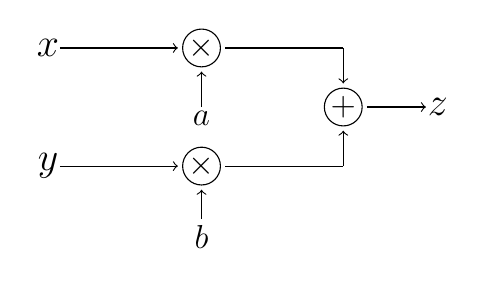
\begin{tikzpicture}[scale=1.5]
        \draw(0,0)node{\Large$x$};
        \draw(0,-1)node{\Large$y$};
        \draw(1.3,-0.6)node{\large$a$};
        \draw(1.3,-1.6)node{\large$b$};
        \draw(1.3,0)node{\large$\times$};
        \draw(1.3,-1)node{\large$\times$};
        \draw(2.5,-0.5)node{\large$+$};
        \draw(3.3,-0.5)node{\Large$z$};
        \draw[->](0+0.1,0)--(1.1,0);
        \draw[->](0+0.1,-1)--(1.1,-1);
        \draw[->](1.3,-0.5)--(1.3,-0.2);
         \draw[->](1.3,-1.45)--(1.3,-1.2);
        \draw(1.5,0)--(2.5,0);
        \draw(1.5,-1)--(2.5,-1);
        \draw[->](2.5,0)--(2.5,-0.5+0.2);
        \draw[->](2.5,-1)--(2.5,-0.5-0.2);
        \draw[->](2.7,-0.5)--(3.2,-0.5);
        \draw(1.3,0) circle (0.16cm);
        \draw(1.3,-1) circle (0.16cm);
        \draw(2.5,-0.5) circle (0.16cm);
    \end{tikzpicture}
    \caption{block ex}
    \label{fig_block_ex}
\end{figure}
\subsection{線形システム}
\subparagraph{インパルス応答}
$$h(t)=L\{\delta(t)\}$$
インパルス信号を入力したときの応答
\subsubsection{周波数応答と伝達関数}
\subparagraph{伝達関数}
$$H(\omega)=G(\omega)e^{j\theta(\omega)}$$
ただし、$G(\omega)$は利得、$\theta(\omega)$は位相シフトを表す。
$$L\{e^{j\omega t}\}=H(\omega)e^{j\omega t}$$
これは、周波数応答を表す式に他ならない。
\subparagraph{周波数応答 $Y(\omega)=H(\omega)X(\omega)$}\leavevmode\\
周波数応答とは、Fig.\ref{fig_H}である。
\begin{figure}[ht]
    \centering
    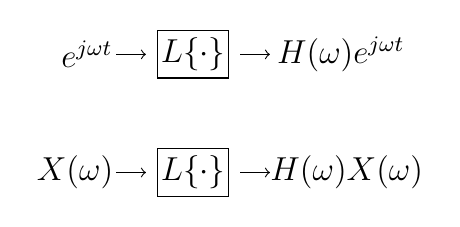
\begin{tikzpicture}[scale=1.5]
        \draw(0,0)node{\large$e^{j\omega t}$};
        \draw(1.8/2,0)node{\large$L\{\cdot\}$};
        \draw[->](0.25,0)--(0.5,0);
        \draw[->](1.3,0)--(1.55,0);
        \draw(2.15,0)node{\large$H(\omega)e^{j\omega t}$};
        \draw(0.6,0.2)rectangle(1.2,-0.2);

        \draw(-0.1,-1)node{\large$X(\omega)$};
        \draw(1.8/2,-1)node{\large$L\{\cdot\}$};
        \draw[->](0.25,-1)--(0.5,-1);
        \draw[->](1.3,-1)--(1.55,-1);
        \draw(2.2,-1)node{\large$H(\omega)X(\omega)$};
        \draw(0.6,0.2-1)rectangle(1.2,-0.2-1);
    \end{tikzpicture}
    \caption{frequency response}
    \label{fig_H}
\end{figure}
すなわち、周波数応答とは正弦波を入力したときの応答と言える。
\subsection{応答と伝達関数}
\begin{itemize}
    \item \textbf{インパルス応答}:時間領域でのシステムの表現
    \item \textbf{周波数応答}:周波数領域でのシステムの表現 
    \item \textbf{伝達関数}:周波数領域における入出力関係
\end{itemize}
\subsection{Fourier変換}
\subparagraph{Fourier級数}
\begin{align*}
x_T(t)&=\sum _{\textcolor{blue}{k=}-\infty} ^{\infty} {C_{\textcolor{blue}{k}} e^{j\textcolor{red}{2\pi\frac{\textcolor{blue}{k}}{T}t}}}\\
C_k&=\frac{1}{T}\int_{\textcolor{red}{-T/2}}^{\textcolor{red}{T/2}}x_{T}(t)e^{-j\textcolor{red}{2\pi\frac{\textcolor{blue}{k}}{T}t}}dt
\end{align*}
\subparagraph{Fourier変換}
$$X(\omega)=\int_{-\infty}^{\infty}x(t)e^{-j\omega t}dt$$
\subparagraph{逆Fourier変換}
$$x(t)=\frac{1}{2\pi}\int_{-\infty}^{\infty}X(\omega)e^{j\omega t}d\omega$$
\subsection{章末問題}
$$\frac{1}{2\pi}\int_{-\infty}^{\infty}e^{j(\omega'-\omega)t}dt=\delta(\omega-\omega')$$
$(\omega'-\omega)$の処理をする際に使いがち(主観)
\section{Laplace変換}
試験範囲外なので省略
\section{アナログからディジタルへ}
\subsection{サンプリング定理}
$$f_{max}\leq\frac{f_s}{2}$$
\subparagraph{ナイキスト周波数$f_N$}
$$f_N=\frac{f_s}{2}$$
\subparagraph{sinc関数}
\begin{itemize}
    \item $\frac{\pi}{2k}$ ($k$は整数)で0になる。
    \item $\mathrm{sinc}(x)=\sin(x)/{x}$のグラフ(Fig.\ref{fig_sinc})
\end{itemize}
\begin{figure}[ht]
    \centering
    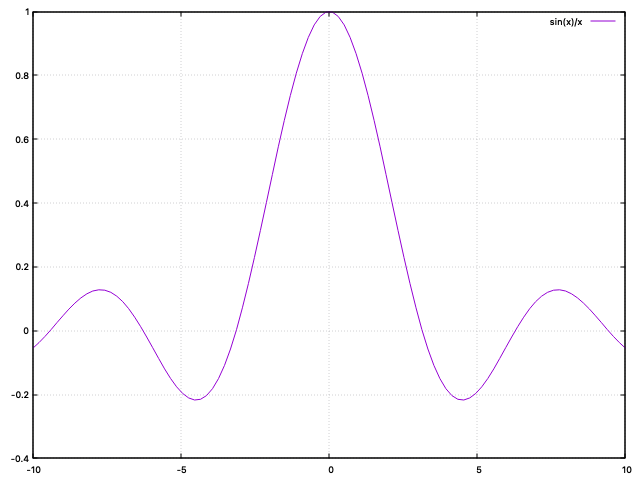
\includegraphics[width=0.3\textwidth]{./fig/fig_sinc.png}
    \caption{sinc}
    \label{fig_sinc}
\end{figure}
\subsubsection{サンプリング定理の一般化(帯域信号)}
$$f_s<f_U-f_L$$
\subsection{SN比}
\subparagraph{最大振幅}
\begin{align*}
\frac{2a_{max}}{\Delta}&=2^n\\
\therefore a_{max}&=\frac{2^n\Delta}{2}
\end{align*}
\subparagraph{信号のパワー}
\begin{align*}
S_{max}&=(\frac{a_{max}}{\sqrt{2}})^2\\
&=2^{2n-3}\Delta^2
\end{align*}
\subparagraph{単位周波数あたりの量子化雑音のパワー}
$$Q_d=\frac{\Delta^2/12}{f_s/2}=\frac{\Delta^2}{6f_s}$$
\subparagraph{量子化雑音のパワー}
$$Q=Q_df_B=\frac{\Delta^2f_B}{6f_s}$$
\subparagraph{SN比のBとdB表記}\leavevmode\\
B(ベル)というのは、\\
\centerline{\textbf{10倍すると1[B](=10[dB])増える単位}}
である。すなわち、SN比のB表記は
\begin{align*}
10^n&=\frac{S_{max}}{Q}\\
\log_{10}10^n&=\log_10\frac{S_{max}}{Q}\\
n[\mathrm{B}]&=\log_{10}\frac{S_{max}}{Q}
\end{align*}
これをdB表記にすると
$$10n[\mathrm{dB}]=10\log_{10}\frac{S_{max}}{Q}$$
これを計算していくと
\begin{align*}
10\log_{10}(\frac{S_{max}}{Q})
&=10\log_{10}(\frac{2^{2n-3}\Delta^2}{\Delta^2f_B/6f_s})\\
&=10\log_{10}(2^{2n-2}\frac{3f_s}{f_B})
% &\fallingdotseq 6n+1.8
\end{align*}
ただし、それぞれの文字は以下の通りである。
\begin{description}
    \item[$f_s$]サンプリング周波数
    \item[$f_B$]周波数帯域幅
    \item[$\Delta$]量子化幅
    \item[$n$]量子化bit数
    \item[$a_{max}$]最大振幅     
\end{description}
\subsection{オーバーサンプリングなしの場合}
オーバーサンプリングなしの場合とは、
\textbf{信号領域が直流からナイキスト周波数$\frac{f_s}{2}$までのとき}
のことである。また、このとき、SN比は
$$6n+1.8$$に近似される。
\subsection{SN比計算における参考値}
\begin{align*}
    \log_{10}2&=3[\mathrm{dB}]\\
    \log_{10}3&=4.771[\mathrm{dB}]
\end{align*}

\clearpage
\part*{補充問題}
\section{線形システム、インパルス応答、伝達関数、周波数応答}
\subsection{インパルス応答の定義}
インパルス応答$h(t)$の定義を書け。
\ans{$$h(t)=L\{\delta(t)\}$$}
\subsection{連続時間システムのインパルス応答}\label{yhx}
出力$y(t)$を入力$x(t)$とインパルス応答$h(t)$を使って書け。
\ans{
\begin{align*}
y(t)=\int_{-\infty}^{\infty}x(t')h(t-t')d\textcolor{red}{t'}
\end{align*}
}
\subsection{インパルス応答}
インパルス応答を言葉で説明せよ。
\ans{インパルス信号$\delta(t)$を入力したときの応答}
\subsection{インパルス応答とConvolution}\label{yhx_c}
\ref{yhx}で求めた関係式をConvolutionを使って書け。
\ans{$$y(t)=x(t)*h(t)$$}
\subsection{インパルス応答を求める。}
インパルス応答を求める方法を具体的に書け。
\ans{
    インパルス応答を求める際は、\ref{yhx}を使うことが基本である。
    具体的には、以下の手順に沿って求める。
    \begin{enumerate}
        \item 入出力関係を求める。
        \item 入出力関係の式を\ref{yhx}の形にする。
    \end{enumerate}
}
\subsection{インパルス応答の具体例}
$y(t)=ax(t)+bx(t-t_0)$のインパルス応答を求めよ。
\subsubsection{インパルス応答を求める(補充問題)}
$$f(t)*\delta(t-t_0)=f(t-t_0)$$が成り立つことを示せ。
\ans{
    $$f(t)*\delta(t-t_0)=f(t-t_0)$$
    の証明については、各自の演習に任せることとする。
    \begin{enumerate}
        \item 入出力関係を求める。
        \item 入出力関係の式を\ref{yhx}の形にする。
    \end{enumerate}
    の手順に従って、進めていく。入出力関係は、仮定より、
    $$y(t)=ax(t)+bx(t-t_0)$$
    よって、これを連続システムにおけるインパルス応答
    $$y(t)=\int_{-\infty}^{\infty}x(t')h(t-t')d\textcolor{red}{t'}$$
    の形になるように変形していく。
    \begin{align*}
        y(t)&=ax(t)+bx(t-t_0)\\
        y(t)&=\int_{-\infty}^{\infty}x(t')h(t-t')dt'\\
        &=x(t)*h(t)
    \end{align*}
    の2つを
    $$f(t)*\delta(t-t_0)=f(t-t_0)$$
    が成り立つことを含めて見比べると、
    $$h(t)=a\delta(t)+b\delta(t-t_0)$$
    となることがわかる。
}

\subsection{Fourier変換のConvolution則}\label{YHX}
Fourier変換のConvolution則を示し、\ref{yhx_c}を変形せよ。
\ans{Fourier変換のConvolution則の証明は省略(教科書の章末問題を要参照)\\
\ref{yhx_c}の両辺をFourier変換すると
$$Y(\omega)=H(\omega)X(\omega)$$
となる。
なお、ここで出てきた$H(\omega)$を伝達関数という。
}
\subsection{線形システム$L\{\cdot\}$}\label{yLx}
線形システムの定義を$y(t),x(t)$を使って書け。
\ans{
    $$y(t)=L\{x(t)\}$$
}
\subsection{伝達関数}\label{H}
伝達関数の定義を書け。
\ans{
    $$H(\omega)=G(\omega)e^{j\theta(\omega)}$$
}
\subsection{周波数応答}
周波数応答を言葉で説明せよ。
\ans{正弦波$e^{j\omega t}$を入力したときの応答}
\subsection{なぜ正弦波を使うか}
線形システム解析において正弦波を使う理由を考えよう。
\subsubsection{正弦波を入力したときの特徴}\label{sin}
線形かつシフト不変なシステムに正弦波を入力したときの特徴を答えよ。
\ans{
    同じ周波数の正弦波が出力される。
}
\subsubsection{正弦波を使う理由}
\ref{sin}を参考にして、正弦波を使う理由を答えよ。
\ans{
    正弦波を入力信号とするとき、、入力信号と出力信号の中で同じ周波数を持つ成分同士が
    1対1に対応する。すなわち、入出力関係においては、
    \begin{itemize}
        \item その振幅が何倍になったか(利得)
        \item 位相がどれだけずれたか(位相シフト)
    \end{itemize}
    のみを考えれば良い。
    また、正弦波は複素指数関数で表せるため、入出力関係を比例関係と表せる。
    よって、数学的な扱いが容易であることも挙げられる(周波数応答の原理)。
}
\subsection{周波数応答}\label{He}
\ref{H}から周波数応答の式を書け。
\ans{
    $$L\{e^{j\omega t}\}=H(\omega)e^{j\omega t}$$
}
\subsection{線形システムと伝達関数}
\ref{yLx}と\ref{He}から\ref{YHX}と同様の式を導け。
\ans{
    \ref{yLx}より$$y(t)=L\{x(t)\}$$
    両辺をFourier変換すると、
    \begin{align*}
        \mathcal{F}[y(t)]&=Y(\omega)\\
        \mathcal{F}[L\{x(t)\}]&=L\{\int_{-\infty}^{\infty}x(t)e^{-j\omega t}dt\}\\
        &=\int_{-\infty}^{\infty}x(t)L\{e^{-j\omega t}\}dt
    \end{align*}
    \ref{He}より$$L\{e^{j\omega t}\}=H(\omega)e^{j\omega t}$$
    よって、
    \begin{align*}
        \mathcal{F}[L\{x(t)\}]&=\int_{-\infty}^{\infty}x(t)H(\omega)e^{-j\omega t}dt\\
        &=H(\omega)\int_{-\infty}^{\infty}x(t)e^{-j\omega t}dt\\
        &=H(\omega)X(\omega)
    \end{align*}
    以上より、
    $$Y(\omega)=H(\omega)X(\omega)$$
}
\subsection{応答と伝達関数}
インパルス応答と周波数応答の関係を示し、伝達関数について説明せよ。
\ans{
    インパルス応答とは、\textbf{時間領域における}システムの表現方法であり、
    周波数応答とは、\textbf{周波数領域における}システムの表現方法である。
    一方、伝達関数とは\textbf{周波数領域における}入出力関係を表すものとなっている。
    また、インパルス応答$h(t)$と周波数応答$H(\omega)$には、以下の関係がある。
    $$\mathcal{F}[h(t)]=H(\omega)$$
}
\subsection{線形性と時不変性}

\clearpage
\section{サンプリング}
\subsection{サンプリング定理}
サンプリング定理を$f_{max},f_s$がそれぞれ何を表すかを説明した上で書け。
\ans{
    $f_{max},f_s$はそれぞれ
    \begin{description}
        \centering
        \item[$f_{max}$]信号の最大周波数
        \item[$f_s$]サンプリング周波数  
    \end{description}
    を示し、サンプリング定理は
    $$f_{max}\leq\frac{f_s}{2}$$
    となる。
}
\subsection{ナイキスト周波数}
ナイキスト周波数$f_N$の定義を書け。
\ans{$$f_N=\frac{f_s}{2}$$}
\subsection{SN比}
SN比を表す式を[dB]で導け。
\ans{
    最大振幅を$a_{max}$、サンプリング周期を$\Delta$、
    bit数を$n$とおくと、
    \begin{align*}
        \frac{2a_{max}}{\Delta}&=2^n\\
        a_{max}&=\frac{2^n\Delta}{2}
    \end{align*}
    となる。よって、波のパワー$S_{max}$は
    \begin{align*}
        s_{max}&=\left(\frac{a_{max}}{\sqrt{2}}\right)^2\\
        &=\frac{2^{2n}\Delta^2}{2^3}\\
        &=2^{2n-3}\Delta^2
    \end{align*}
    となる。一方、量子化雑音単位周波数あたりのパワー$Q_d$は
    $$Q_d=\frac{\Delta^2}{6f_s}$$
    となる。よって、最大周波数が$f_B$であるとき量子化雑音のパワー$Q$は
    \begin{align*}
        Q&=Q_df_B\\
        &=\frac{\Delta^2f_B}{6f_s}
    \end{align*}
    SN比とは、$S_{max}/Q$であり、B(ベル)とは、10倍すると1増える単位であることから
    ベルを$x$とおくと
    \begin{align*}
        10^x&=S_{max}/Q\\
        &=\frac{2^{2n-3}\Delta^2}{{\Delta^2f_B}/{6f_s}}\\
        &=3\cdot2^{2n-2}\frac{f_s}{f_B}\\
    \end{align*}
    \begin{align*}
        x&=\log_{10}\left(3\cdot2^{2n-2}\frac{f_s}{f_B}\right) \; [\mathrm{B}]\\
        &=10\log_{10}\left(3\cdot2^{2n-2}\frac{f_s}{f_B}\right) \; [\mathrm{dB}]\\
    \end{align*}
    となる。
}
\subsection{SN比とナイキスト周波数}
信号の最大周波数がナイキスト周波数であり、n[bit]の情報を格納できる際の
最大SN比を求めよ。
\ans{
    6n+1.8
}

\nocite{*}
\printbibliography

\end{document}